\section{一种新的亚线性PIR构造方案}
在本小节中,我们提出了一种新的设计,用于构建一个高效的两服务器PIR方案,该方案避免了使用虚设查询,同时保持了查询的效率仍是亚线性的。
我们遵循前文提到的协议,并尝试通过三种优化技术来解决上述问题:(i) 使用“划分与采样”技术实现高效的隶属测试,(ii) 使用伪随机函数压缩集合以提高空间和通信效率,(iii) 通过一个新的概念 Crumb 隐藏查询索引。以下是这些技术的详细说明:
\subsection{对数据库进行划分}

\begin{figure*}
    \begin{subfigure}{0.5\textwidth}
        \centering
        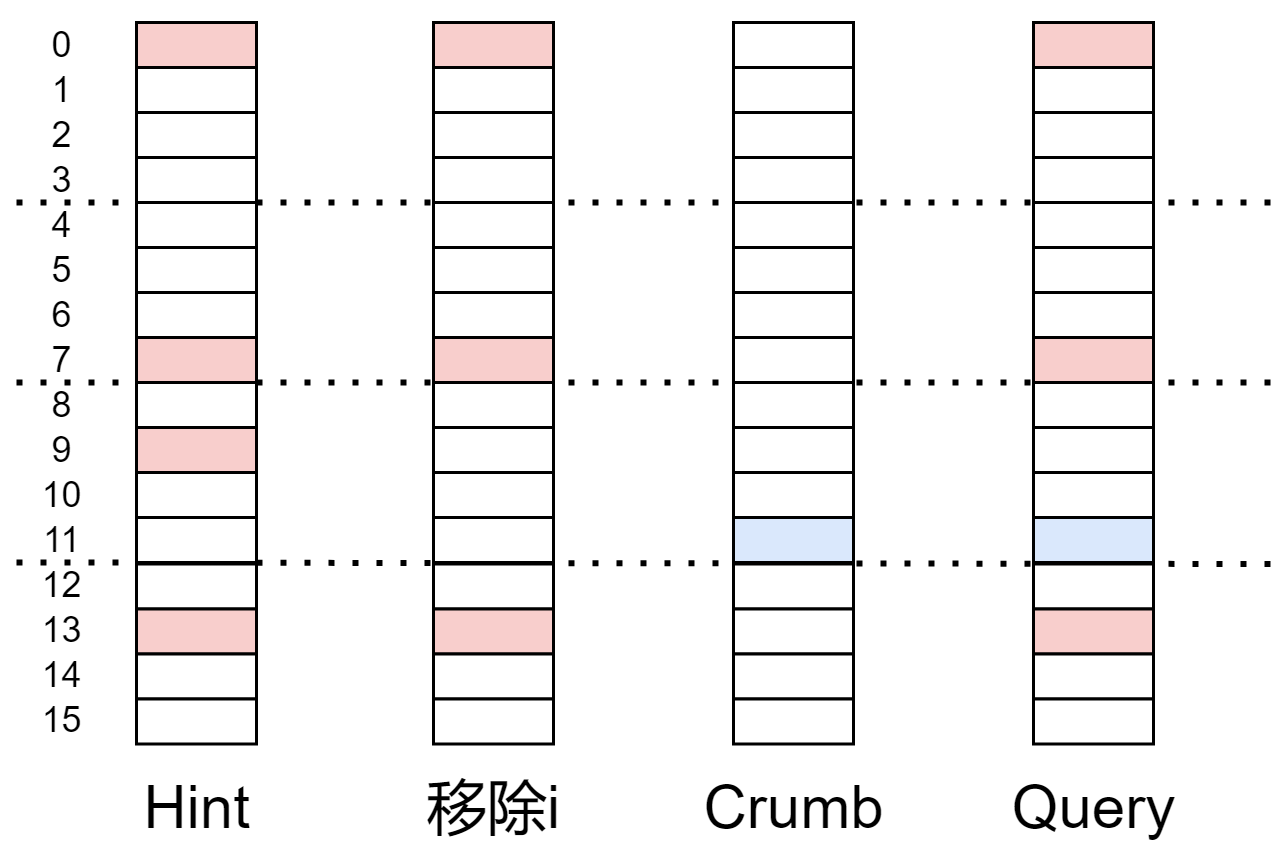
\includegraphics[width=0.8\linewidth]{figure/sketch1.png}
        \caption{Query construction} \label{fig:query-a}
    \end{subfigure}%
    \hspace*{\fill}   % maximize separation between the subfigures
    \begin{subfigure}{0.5\textwidth}
        \centering
        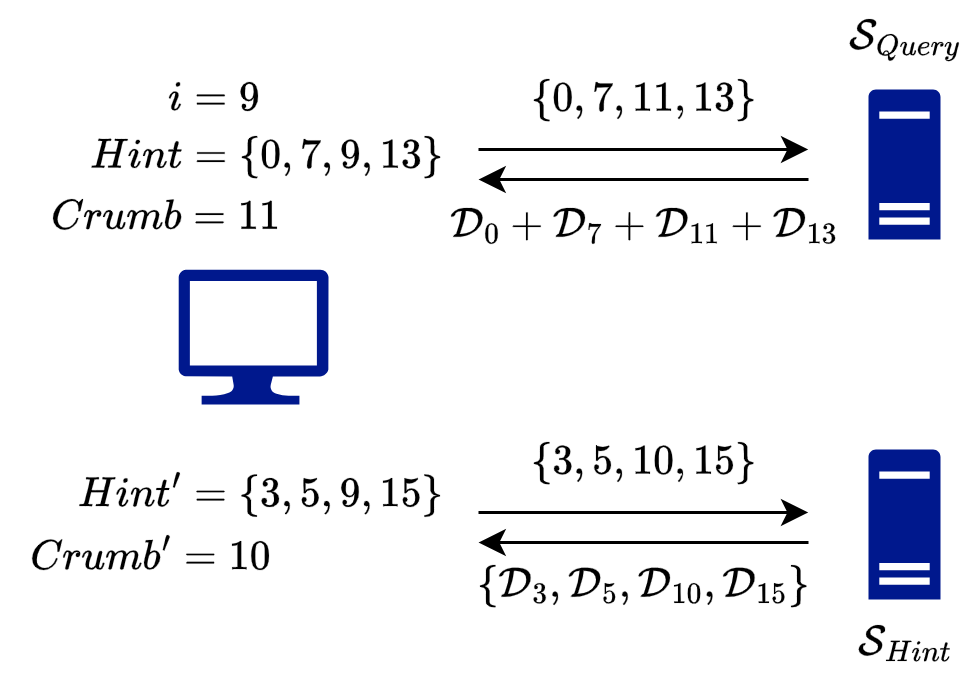
\includegraphics[width=0.8\linewidth]{figure/sketch2.png}
        \caption{Query process} \label{fig:query-b}
    \end{subfigure}%
    \caption{一次查询的示例。数据库包含$\dbsize=16$条记录,并被划分为$\sqrt{\dbsize}=4$个区块。 \hyperref[fig:query-a]{a)} $Hint$包含每个区块中的一个条目(图中标记为红色)。客户端希望查询记录$\dbidx=9$,该记录位于第三个区块。该索引从集合中移除(在第二列中显示),并在第三个区块中添加了一个Crumb到集合中(第三列和第四列标记为蓝色)。 \hyperref[fig:query-b]{b)} Query服务器以集合的校验值作为响应。客户端生成一个新的Hint集合以更新Hint和Crumb。Hint服务器以单条记录作为响应。为作说明目的,索引在此处以明文表示,实际在区块中以偏移量表示。}
    \label{fig:query}
\end{figure*}

在前文的协议中,每个集合$\setkey_j, j\in[\hintcount]$的索引都是随机生成的,这阻碍了高效的隶属测试。借鉴现有文献 \cite{Piano, C:LazPap23} 的启发,我们采用了一种将数据库分成$\sqrt{\dbsize}$个块的方法,每个块包含$\sqrt{\dbsize}$条记录。我们通过以下方式生成每个集合 $S$:
为每个块 $j$ 随机生成一个偏移量$x_j \leftarrow [\sqrt{\dbsize}], j \in [\sqrt{\dbsize}]$,通过这些偏移量计算出实际集合$S=\{x_j+j\cdot \sqrt{\dbsize} \mid j \in [\sqrt{\dbsize}]\}$。

这种方法能够实现高效的隶属测试。为了确定查询的索引$\dbidx$是否在集合$S$中,客户端会计算集合$S$中第$\lfloor \dbidx/\sqrt{\dbsize}\rfloor$项,并检查它是否等于$\dbidx-\sqrt{\dbsize}\cdot\lfloor \dbidx/\sqrt{\dbsize}\rfloor$。这种取集合中“第x项”的操作要求集合必须保持\textbf{有序},以便确定一个偏移量属于哪个块。为了简化表示,我们假设集合可以像向量一样进行排序和索引。

在这种方案下,每个集合不再是完全随机生成的。一个集合一定由每个块中的一个元素组成。一个集合既不可能包含一个块中的两个元素,也不可能跳过某个块。我们已经享受到了这种结构给我们带来了好处:它使得隶属测试变得很简单。然而,这种集合组成也会带来一定的问题,我们将在 \ref{sec:problem-of-dividing} 节中讨论。


\subsection{优化存储方案}
先前的工作~\cite{EC:CorKog20, C:LazPap23} 选择使用可打孔的伪随机函数(Puncturable Pseudorandom Function)来压缩集合,从而减少通信成本。然而,在实践中,可打孔伪随机函数这一原语开销比较高,因为它计算集合的效率比较低。相反,我们选择了普通的伪随机函数。具体来说,指定一个由密钥$\setkey$参数化的伪随机函数族,即$f_{\setkey}: [\sqrt{\dbsize}] \to [\sqrt{\dbsize}]$,我们就可以使用一个长度为 $\lambda$ 的密钥$\setkey$表示一个集合 $S$:$$S = \{f_{\setkey}(j) + j \cdot \sqrt{\dbsize} \mid j \in [\sqrt{\dbsize}]\}$$ 其中$\lambda$ 是计算安全参数。由此,隶属测试可以表示为:$$f_{\setkey}(\lfloor i/\sqrt{\dbsize}\rfloor) = i - \sqrt{\dbsize}\cdot\lfloor i/\sqrt{\dbsize}\rfloor$$。

在实践中,这一方案还包括一个额外的偏移量 $\shift$。该偏移量对集合中的每个元素进行了一次置换(这一技术也在文献 \cite{EC:CorKog20, C:LazPap23} 中使用)。具体来说,集合现在表示为$S = \{(f_{\setkey}(j)\oplus \shift) + j \cdot \sqrt{\dbsize} \mid j \in [\sqrt{\dbsize}]\}$(其中$\oplus$表示异或操作)。有了这一偏移量之后,我们可以在 $O_\lambda(1)$ 时间内,以确定性的方式生成包含给定索引 $\dbidx$ 的集合。具体做法是先生成一个密钥$\setkey$,并将偏移量设置为$\shift \coloneqq f_{\setkey}(\lfloor \dbidx/\sqrt{\dbsize}\rfloor) \oplus (i - \sqrt{\dbsize}\cdot\lfloor i/\sqrt{\dbsize}\rfloor)$。如果没有特定索引需要包含,则偏移量可以从$[\sqrt{\dbsize}]$中随机生成。我们使用$Eval(\setkey,\dbidx)$来简写$f_{\setkey}(\dbidx)\oplus \shift + \dbidx\cdot\sqrt{\dbsize}$。为了使表达式不至太过复杂,我们假设在计算集合时总是包含了偏移量,但在后续讨论中省略关于偏移量的符号。

为了符号简洁考虑,我们将把密钥 $\setkey$ 展开为集合 $S$ 的过程记作 $S = Expand(\setkey)$。

通过放弃可打孔的伪随机函数,我们实现了显著的性能提升。然而,这一变更的代价是,从集合中删除元素之后,集合就无法使用较短的一个密钥表示了。此时,我们要求协议的参与方通过非压缩的方式,直接传输集合的每个元素。客户端在离线时以$O_\lambda(1)$ 大小保留并传输密钥,并在在线时以$O(\sqrt{\dbsize})$的通信量发送非压缩集合。

\subsection{优化查询方案}
\label{sec:problem-of-dividing}
对数据库进行划分提高了隶属测试的效率。然而,它也带来了一个新的问题:由于每个块中固定有且仅有一个元素,很容易就能从删去一个元素的集合推断出删去的元素落在哪个块中。对应到PIR应用中,服务器可以知道客户端想要查询的索引落在哪个块里,这显然不符合隐私性的要求。我们需要一种新方案,能隐藏被删除的索引。为了解决这一问题,我们提出一种新的Hint信息,称为Crumbs。一个 Crumb $\crumb=(\crumbvalue, \crumboffset)$ 由一条记录的值 $\crumbvalue$ 及其在块中的位置 $\crumboffset$ 组成。在离线阶段,客户端从每个块中获取一个随机的Crumb,总共会得到 $\sqrt{\dbsize}$ 个。

这一做法的核心思路是用 Crumb 来“掩盖”被删去的元素。具体来说,当客户端希望查询第 $\dbidx$ 条记录时,它首先找到一个包含 $\dbidx$ 的集合 $S$。在从集合中找到 $\dbidx$ 后(由于集合划分的性质,$\dbidx$应该落在第$\blockidx = \lfloor \dbidx/\sqrt{\dbsize} \rfloor$ 块中),它会在第 $\blockidx$ 块中找到一个 Crumb $\crumb=(\crumbvalue, \crumboffset)$,并将第$\blockidx$块对应的偏移替换为 $\crumboffset$ 。这个过程如图 \ref{fig:query} 所示。

用于替换的Crumb不会影响客户端计算答案。由于每个Crumb仅包含一个简单的记录,因此可以很容易地通过排除Crumb的贡献来计算真实答案。具体来说,假设$\answer$是来自服务器的答案,$\crumbvalue$是所用Crumb的值,客户端计算$\answer \coloneqq \answer - \crumbvalue$。最后,客户端可以按照原本协议中的方式重构记录$\db_\dbidx$。

容易看出,Crumb很好地掩盖了客户端想要查询的位置。客户端发送给服务器的集合现在由每个块中的一个随机偏移量组成,与查询的索引$\dbidx$完全无关。我们的构造保持了亚线性效率:在离线阶段,客户端接收到大小为$\recordsize\hintcount$的Hint,这些信息由服务器在$O_\lambda(\recordsize\sqrt{\dbsize}\hintcount)$时间内计算。假设$\hintcount\coloneqq \Theta_\lambda(\sqrt{\dbsize})$,当这一计算均摊在$\querycount\coloneqq\Theta_\lambda(\sqrt{\dbsize})$次在线查询上时,每次查询的通信开销为$O(\recordsize\sqrt{\dbsize})$,计算开销为$O_\lambda(\recordsize\sqrt{\dbsize})$。

我们特别指出,在我们的方案中,没有使用虚构查询。这种方法使我们能够实现有效的验证,详细内容将在第 \ref{sec:verifiable} 节中介绍。

\subsection{Hint的获取与更新}
Hint的获取与更新也是离线-在线PIR方案中的关键环节。有几个显然的要点,我们在设计方案时必须考虑到:
\begin{itemize}
    \item 每条记录都需要至少在某一个Hint集合内,否则,在在线阶段查询该记录将无法实现。
    \item 方案必须支持超过一定数量的在线查询,以将昂贵的离线成本分摊到这些在线查询上。
    \item 客户端不能重复使用一个Hint,否则服务器通过对比这些Hint就能获得关于查询索引的信息。因此,Hint在一次使用后必须被丢弃。
\end{itemize}

离线阶段的Hint和Crumb的获取并不困难的。鉴于服务器$\hintserver$是半诚实的,所有Hint都可以从客户端提供的一个PRF密钥中生成,服务器计算相应的校验值后发送给客户端。Crumb也可以通过相同的方式获取。

在线阶段的Hint和Crumb更新则需要更复杂的交互。在原本的协议中,更新是通过客户端生成一个包含查询索引$\dbidx$的新集合,并与服务器$\hintserver$交互以获取该集合的Hint来完成的。这一过程也需要隐藏$\dbidx$。理所应当地,我们会想要使用与查询类似的手段,用一个Crumb来掩盖住$\dbidx$。然而,在我们的协议中,Crumb就是从$\hintserver$获取的,不能再用于保护向$\hintserver$发送的请求。否则,$\hintserver$可以通过比较查询和Crumb,得知哪个块被Crumb替换了。

为了解决这一矛盾,我们采用一种不同于查询的方案来更新Hint。客户端仍然生成一个包含查询索引$\dbidx$的新集合$S'$,但是选择一个随机的索引$j$来替换块$\blockidx$中的$\dbidx$。当然,如果$\hintserver$仅以一个校验值响应查询,客户端将无法获知$\db_{j}$是什么,也就没有办法获得原集合$S'$对应的校验值。为了使客户端能够将协议进行下去,$\hintserver$必须直接将收到的查询中包含的 $\sqrt{\dbsize}$ 条记录全部发送给客户端。客户端则通过这$\sqrt{\dbsize}$条记录与之前查询得到的$\db_\dbidx$更新Hint,并使用$\db_{j}$来更新用掉的Crumb。采用这种Hint和Crumb更新方案后,我们的方案现在能够支持多项式数量的查询,这与最近在文献 \cite{C:LazPap23} 中所达成的进展一致。关于正确性的讨论将延后到第 \ref{sec:analysis} 节。完整的协议见图 \ref{fig:two-server}。

\begin{figure}
    \begin{mdframed}
        \centering
        \textbf{两服务器协议}

        \raggedright
        \paragraph{符号约定:} 协议包含一个客户端 $\client$,一台Query服务器 $\queryserver$ 与一台Hint服务器 $\hintserver$。单个Hint由元祖:$\hint=(\setkey,\sumhint)$构成。单个Crumb包含了一个偏移量和一条记录值 $\crumb=(\crumboffset,\crumbvalue)$。$fk_{key}:\{0,1\}^\lambda \to \{0,1\}^\lambda$ 是一个能将单一PRF密钥映射为多个PRF密钥的PRF函数, $f_{\setkey}: [\sqrt{\dbsize}]\to [\sqrt{\dbsize}]$ 是一个将块序号转化为偏移量的PRF,  $Eval(\setkey,\dbidx) \coloneqq f_{\setkey}(\dbidx)\oplus \shift + \dbidx\cdot\sqrt{\dbsize}$ 与 $Expand$ 密钥 $\setkey$ 标识计算密钥对应的集合内元素 $\{Eval(sk,j) \mid j\in[\sqrt{\dbsize}]\}$. 假设 $\dbidx$ 是需要查询的索引。 在离线阶段,总共生成 $\hintcount$ 个 Hint.

        \paragraph{离线阶段:}
        \begin{itemize}
            \item \textbf{Setup:} $\client$ 生成一个PRF密钥 $mk\in\{0,1\}^\lambda$,将本地的Hint存储初始化为 $\hint_j\coloneqq(fk_{mk}(j),0), j\in [\hintcount]$,Crumb存储初始化为 $\crumb_j\coloneqq (\bot,\bot), j\in [\sqrt{\dbsize}]$。 $\client$ 将 $mk$ 发送给 $\hintserver$.
            \item \textbf{Hint:}
                  \begin{itemize}
                      \item $\hintserver$ 将 $mk$ 展开为PRF密钥 $\setkey_j=fk_{mk}(j), j\in[\hintcount]$ 。它将这些密钥进一步$Expand$为集合 $S_j, j\in[\hintcount]$。
                      \item $\hintserver$ 为每个集合计算校验值 $\sumhint_j\coloneqq \sum_{k\in [\sqrt{\dbsize}]}\db_{S_{j}[k]}, j\in[\hintcount]$ 。$\hintserver$将这些校验值发送给 $\client$。
                      \item 在第 $j$ 个 $\sqrt{\dbsize}$ 大小的块 ($j\in[\sqrt{N}]$) 内, $\hintserver$ 随机选取一个偏移量 $\crumboffset_j\leftarrow [\sqrt{N}]$ 及其对应的记录值 $\crumbvalue_j$ 作为Crumb。它将这些Crumb $\crumb_j \coloneqq  (\crumboffset_j, \crumbvalue_j), j\in [\sqrt{\dbsize}]$ 发送给 $\client$。 $\client$ 接受并储存这些Crumb。
                  \end{itemize}
        \end{itemize}
        \paragraph{在线阶段:}
        \begin{itemize}
            \item \textbf{Query ($\queryserver$):}
                  \begin{itemize}
                      \item 记 $\dbidx$ 所在的块为 $\blockidx\coloneqq \lfloor \dbidx/\sqrt{\dbsize}\rfloor$。 $\client$ 在存储中找到一个Hint $\hint_\hintidx = (\setkey_\hintidx,\sumhint_\hintidx)$,满足条件 $f_{\setkey_\hintidx}(\blockidx) = \dbidx-\sqrt{\dbsize}\cdot \blockidx$。如果没有这样的Hint,$\client$ 终止查询并输出 $\bot$.
                      \item $\client$ 将 $\setkey_\hintidx$ $Expand$ 为集合 $S$。$\client$ 找到 $\blockidx$ 的 Crumb $\crumb_\blockidx=(\crumboffset_\blockidx, \crumbvalue_\blockidx)$,将 $S[\blockidx]$ 替换为Crumb偏移量 $\crumboffset_\blockidx$。  $\client$ 将 $S$  发送给 $\queryserver$.
                  \end{itemize}
            \item \textbf{Answer ($\queryserver$):} $\queryserver$ 计算校验值 $\sumanswer\coloneqq \sum_{k\in [\sqrt{\dbsize}]}\db_{S[k]}$ 。$\queryserver$ 将 $\sumanswer$  发送给 $\client$.
            \item \textbf{Reconstruct:} $\client$ 重构出记录 $\db_\dbidx \coloneqq  \sumhint_\hintidx-(\sumanswer-\crumbvalue_\blockidx)$。  $\client$ 输出 $\db_\dbidx$。
            \item \textbf{Query ($\hintserver$):}
                  \begin{itemize}
                      \item $\client$ 生成PRF密钥 $\setkey'$ 使得 $f_{\setkey'}(\blockidx) = \dbidx-\sqrt{\dbsize}\cdot \blockidx$。 .
                      \item $\client$ 将 $\setkey'$ $Expand$ 为集合 $S'$。$\client$ 将 $S'[\blockidx]$ 替换为随机偏移 $\crumboffset' \leftarrow [\sqrt{\dbsize}]$. $\client$ 将 $S'$ 发送给 $\hintserver$.
                  \end{itemize}
            \item \textbf{Answer ($\hintserver$):} $\hintserver$ 直接将 $\sqrt{\dbsize}$ 条记录 $\db_{S'[j]}, j\in [\sqrt{\dbsize}]$ 发送给 $\client$。
            \item \textbf{Refresh:} $\client$ 将Crumb更新为 $\crumb_\blockidx \coloneqq  (\crumboffset', \db_{S'[\blockidx]})$,将Hint更新为 $\hint_\hintidx \coloneqq  (\setkey',\db_\dbidx + \sum_{k\in [\sqrt{\dbsize}],k\neq \blockidx}\db_{S'[k]}, )$
        \end{itemize}
    \end{mdframed}
    \caption{两服务器PIR协议。向$\queryserver$ 和 $\hintserver$ 进行 $Query$ 的算法仅为清晰起见进行了分离。它们可以并行运行,不需要额外的轮次。}
    \label{fig:two-server}
\end{figure}